\documentclass[12pt,a4paper]{report}
\usepackage[utf8]{inputenc} % this is needed for umlauts
\usepackage[ngerman]{babel} % this is needed for umlauts
\usepackage[T1]{fontenc}    % this is needed for correct output of umlauts in pdf

\usepackage{ucs}
\usepackage{amsmath}
\usepackage{amsfonts}
\usepackage{amssymb}
\usepackage{graphicx}

\usepackage{hyperref}
\usepackage{csquotes}
\usepackage{appendix}
\usepackage{pdfpages}
\usepackage{float}

\begin{document}

	\tableofcontents
	\newpage
	
	\chapter{Vorwort}
	Dieses Dokument findest du auf github.com unter: \href{https://github.com/henri-libre/analysis1}{https://github.com/henri-libre/analysis1}. Du darfst das Dokument nutzen, erweitern und verbreiten. Maintainer des Dokumentes erreichst du entweder dort oder per E-Mail an \href{analysis1istgeil@nanooq.org}{analysis1istgeil@nanooq.org}. Für die Korrektheit des Dokumentes ist entweder keiner oder du verantwortlich. Die URL der Veranstaltung an sich lautet: \href{https://analysis3.wordpress.com/analysis-i-ws-1516/uebungen-zu-analysis-i-wise-1516/}{https://analysis3.wordpress.com/analysis-i-ws-1516/uebungen-zu-analysis-i-wise-1516/}
	
\chapter{Übungsblatt 1}
	
	Das entsprechende Übungsblatt befindet sich im Anhang \ref{uebungsblatt1}.
	
	\section{Aufgabe 1: Vollständige Induktion}
	Beweisen Sie mit vollständiger Induktion: Für alle $ n \in N $ gilt:
	\begin{enumerate}
	\item $ 5^n - 1 $ ist durch 4 teilbar.
	\item $ 3^{2^n} - 1 $ ist durch $ 2^(n+2)$ teilbar.
	\item Die Anzahl $A_n$ aller Teilmengen einer $n$-elementigen Menge ist gegeben durch $A_n=2^n$
	\end{enumerate}
	
	\subsection{Musterlösung}
	Noch nicht bekannt gegeben
	
	\subsection{Lösung Lerngruppe \enquote{HenriLibre, du?, du?, du?}}
	\begin{enumerate}
	\item z.~z.: $5^n - 1 | 4 $ 
		\begin{itemize}
			\item Induktionsanker:\\
			$n_1 = 1: 5^1 - 1 = x \cdot 4$ \\
			$\Leftrightarrow 5-1 = x \cdot 4 $ \\
			$\Leftrightarrow x = 4 $ \\
			\item Induktionsvoraussetzung:\\
			$ (5^n -1)$ ist durch 4 teilbar.\\
			\item Induktionsschritt: \\ 
			$ n \mapsto n+1: a_{n+1} = 5^{n+1}-1$ \\ 
			$ = (5 \cdot 5^n)-1$ \\
			$ (4 \cdot 5^n + 5^n) -1$ \\
			$ (4 \cdot 5^n) + (5^n -1)$\\
			Erster Term ist per Definition durch 4 teilbar. Zweiter Term ist gleich unserer Induktionsvoraussetzung.  
		\end{itemize}
	\item z.~z.: $ 3^{2^n}-1|2^{n+2} $ 
		\begin{itemize}
			\item Induktionsanker:\\
			$ n_1 = 1: 3^2 -1 = 9 - 1 = 8 $
			\item Induktionsvoraussetzung:\\
			$ 3^{2^n} - 1 $ durch $ 2^{n+2} $ teilbar.
			\item Induktionsschritt: \\ 
			$ n \mapsto n+1: 3^{2^{n+1}} -1 \\
			\overset{\text{aus der Kla-}}{\underset{\text{mer ziehen}}{=}} (3^{2^n})^2 -1\\ \overset{\text{Binomische}}{\underset{\text{Formel}}{=}} (3^{2^n}-1)(3^{2^n}+1)$ \\
			Erster Term ist die Induktionsvoraussetzung. Der zweite Term ist im Detail unwichtig, wegen der Multiplikation.
		\end{itemize}
	\item z.~z.: Für Menge $M$ mit $|M| = n \Rightarrow |P(M)|=2^n$
		\begin{itemize}
			\item Induktionsvoraussetzung:\\
			$ n=1: $ Sei $M=\{n\}$. Dann ist $P(M)=\{\varnothing,\{a\}\} \rightarrow |P(M)|=2^1$.
			\item Induktionsschritt:\\
			Dann sei $M^*=\{a_1,\dots, a_n\}$.\\
			Dann gilt laut Induktionsvoraussetzung: $|P(M^*)=2^n|$.
			\\Nun gilt\footnote{$P(M) \setminus P(M^*)$ muss disjunkt sein, weil: Wenn A, B disjunkt, dann $ A \cap B = \varnothing$.} $P(M) \setminus P(M^*) = \{T \cup \{a_{n+1}\} | T \in P(M^*)\} \\
			\Rightarrow |P(M)|=2|P(M^*)|=2\cdot 2^n= 2^{n+1}$
			\item Erklärung:\\
			Es sei $ P(m^*) = \{\varnothing\}, \{a_1\}, \{a_2\}, \{a_1,a_2\}$. Wenn nun $ \{a_3\} $ hinzugefügt wird, ist $ P(m) = P(m^*) \cup \{a_{3}\} = \{\varnothing\}, \{a_1\}, \{a_2\}, \{a_1,a_2\},\\
			\{a_3\}, \{a_1,a_3\}, \{a_2,a_3\}, \{a_1,a_2,a_3\} $.
		\end{itemize}
	\end{enumerate}

\section{Aufgabe 2: Indirekter Beweis}

Es seien $ a_1,\dots, a_m \in N $. Beweisen Sie: Gilt für ein $n \in N $
\begin{equation}
\prod^{m}_{i=1}(1+a_i) > 2^m,\text{so folgt} \sum^{m}_{i=1}a_i > n.
\end{equation}

	\subsection{Lösung Lerngruppe \enquote{HenriLibre, du?, du?, du?}}
	Indirekt: z.z. für $ a_1, \ldots, a_n \text{ mit } n \in N$ gilt\\
	\begin{equation}
	\prod^{m}_{i=1}(1+a_i) > 2^m,\text{so folgt} \sum^{m}_{i=1}a_i > n.
	\end{equation}
	Exkurs \enquote{Indirekter Beweis}: $(A \Rightarrow B) \Leftrightarrow (\neg B \Rightarrow \neg A)$:
	
	\begin{table}[H]
		\center
		\begin{tabular}{c | c | c | c | c }
		 \# & A & B & A $\Rightarrow B $ & $ \neg B \Rightarrow \neg A $ \\
		 \hline
		 1 & f & f & w & w \\
		 2 & f & w & w & w \\
		 3 & w & f & f & f \\
		 4 & w & w & w & w \\
		\end{tabular}
		\caption{ In der dritten Zeile steht der Indirekter Beweis}
		\end{table}
		
	Zunächst zeigen wir: $ (1+k) \leq 2^k $ ~~ $ \forall k \in N$:
	\begin{align*} 
	&n = 1:  1 + 1 = 2 \leq 2^1 = 2\\
	&n = 2:  1 + 2 = 3 \leq 2^2 = 4\\
	&n = 3:  1 + 3 = 4 \leq 2^3 = 8\\
	&n \mapsto n+1:\\
	&1+(n+1) \leq 1+2^n \leq 2+2^n \leq 2^{(n+1)}\\
	&\prod^m_{i=1}(1+a_i)=(1+a_1)\cdot\ldots\cdot (1+a_m) \overset{\text{Hinweis}}{\leq}  2^{a_1}\cdot\ldots\cdot 2^{a_m} = 2^{\sum^{n}_{i=1}a_i} \leq 2^n
	\end{align*}
	
\section{Aufgabe 3: Vollständige Induktion}
\begin{enumerate}
	\item Gegeben sei ein Schachbrett mit der Seitenlänge $2^n$, von dem ein beliebiges Geld entfernt wird. Zeigen Sie, dass das Brett mit \enquote{L}-förmigen Kartonstückchen überdeckt werden kann. Die Kartonstückchen sind dabei so groß, dass sie genau drei Felder bedecken. Die Kartonstücke dürfen sich nicht überlappen.
	\item Zeigen Sie, dass für jede natürliche Zahl $n$ die Zahl $2^{2n}-1$ durch $3$ teilbar.
\end{enumerate}

\subsection{Lösung Lerngruppe \enquote{HenriLibre, du?, du?, du?}}

\begin{enumerate}
	\item Z.~z. dass das Brett mit \enquote{L}-förmigen Kartonstpcken überdecken.
	\begin{itemize}
		\item Induktionsanker:
			\begin{table}[H]
				\centering
				\begin{tabular}{|c|c|c|c|}
					\hline
					~~&~~&~~&~~\\
					\hline
					&&&\\
					\hline
					&&&\\
					\hline
					&&&\\
					\hline
				\end{tabular}
				\caption{Schachbrett mit der Seitenläge $2^n$}
			\end{table}
		\item Induktionsvoraussetzung:\\
		$n=1: 2 \times 2 \rightsquigarrow$ \enquote{L}-förmiges Kartonstückchen $\Rightarrow$ Vollständige Überdeckung.
		
		\item Induktionsschritt:\\
		$n\mapsto n+1$: Wir nehmen von einem Schachbrett mit Seitenlänge $2^{n+1}$ ein Feld weg und teilen es in 4 Schachbretter mit der Seitenlänge $2^n$ auf:
		\begin{table}[H]
			\centering
			\begin{tabular}{|c|c||c|c|}
				\hline
				2 & 2 & 1 & X \\
				\hline
				2 & 2 & 1 & 1 \\
				\hline
				\hline
				3 & 3 & 4 & 4 \\
				\hline
				3 & 3 & 4 & 4 \\
				\hline
			\end{tabular}
			\caption{Schachbrett mit der Seitenläge $2^{n+1} $, das weggenommene Feld sei X}
		\end{table}
		Sei das weggenommene Feld ohne Beschränkung der Allgemeinheit oben rechts aus 1. Dann können wir laut Induktionsvoraussetzung das Feld 1 vollständig überdecken. Genauso können wir dies mit den Feldern 2, 3 und 4 bis auf ein Feld überdecken. Diese drei Felder werden so angeordnet:
		
		\begin{table}[H]
			\centering
			\begin{tabular}{|c|c||c|c|}
				\hline
				2 & 2 & 1 & X \\
				\hline
				2 & L & 1 & 1 \\
				\hline
				\hline
				3 & L & L & 4 \\
				\hline
				3 & 3 & 4 & 4 \\
				\hline
			\end{tabular}
			\caption{}
		\end{table}
		
		Dann können wir diese drei Felder auch überdecken. Dann ist das gesamte Brett mit Ausnahme des weggenommenen Feldes vollständig überdeckt. $ \square $
	\end{itemize}
\item Aus dem ersten Aufgabenteil folgt nicht, dass der Beweis für diesen Aufgabenteil. Viel mehr ist der erste Teil ein Spezialfall von diesem Aufgabenteil.\\
Z.~z.: $ 3|2^{2n}-1$
\begin{itemize}
	\item Induktionsanker:
	\begin{flalign*}
		n_1 = 1: 3 &= 2^{2\cdot 1} - 1 &\\
		\Leftrightarrow 3 &= 4 - 1 &\\
		\Leftrightarrow 3 &= 3
	\end{flalign*}
	\item Induktionsvoraussetzung:\\
	$ 3|2^{2n}-1$
	\item Induktionsschritt:
	\begin{flalign*}
		n \mapsto n+1: 3 &|2^{2(n+1)} - 1 & \\
		\Leftrightarrow 3 &| 2^{2n} \cdot 2^2 - 1 &\\
		\Leftrightarrow 3 &| 2^{2n} \cdot 3
	\end{flalign*}
	Eigentlich müsste der letzte Teil irgendwie durch 3 teilbar sein.
\end{itemize}
\end{enumerate}

\section{Aufgabe 4: Vollständige Induktion}
Wo steckt der Fehler in folgendem induktionsbeweis?\\
Behauptung: für $ n \geq 1 $ gilt: je $n$ natürliche Zahlen sind gleich.\\
Beweis: 
\begin{itemize}
	\item Induktionsanfang: Für $ n = 1 $ ist die Behauptung offensichtliche wahr.
	\item Induktionsschritt: Die Behauptung gelte für $ n \in N$ (Induktionsannahme). betrachte die Menge $\{a_1, a_2, \ldots, a_n, a_{n+1}\}$ von $n+1$ natürlichen Zahlen. Die natürlichen Zahlen $ a_1, a_2, \ldots, a_n$ bzw. $ a_2, a_3, \ldots, a_n, a_{n+1}$ sind nach Induktionsannahme gleich, d.h. $ a_1 = a_2 = \ldots = a_n$ bzw. $ a_2 = a_3 = \ldots = a_{n+1}$. Damit folgt $a_1 = a_2 = \ldots = a_{n+1}$, also die Behauptung. $\square$
\end{itemize}

\appendices
	\chapter{}
	\section{Übungsblatt 1}\label{uebungsblatt1}
	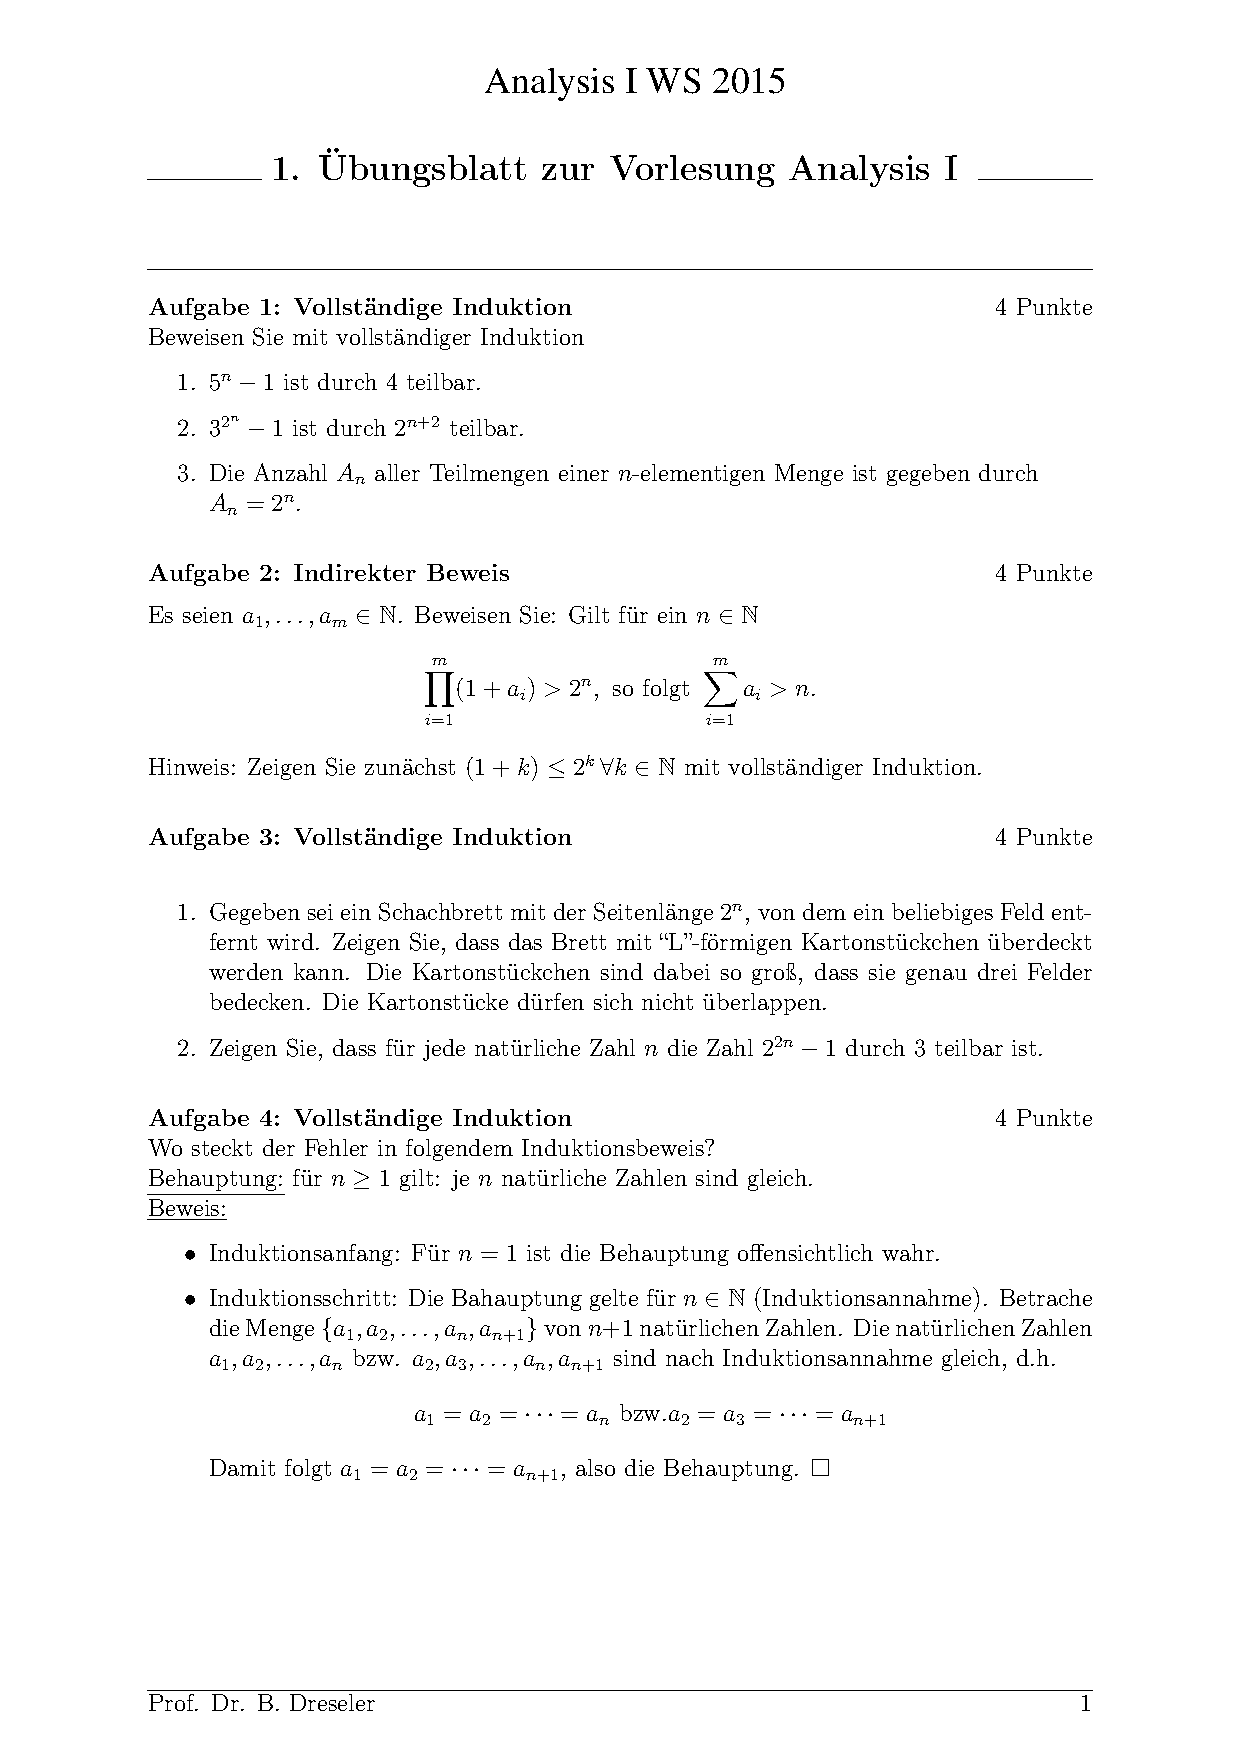
\includepdf[pages=-]{blatt1}
\end{document}